%%%%%%%%%%%%%%%%%%%%%%%%%%%%%%%%%%%%%%%%%%%%%%%%%%%%%%%%%%%%%%%%%%%%%%%%%%%%%%%%
%2345678901234567890123456789012345678901234567890123456789012345678901234567890
%        1         2         3         4         5         6         7         8

\documentclass[letterpaper, 10 pt, conference]{ieeeconf}  % Comment this line out if you need a4paper. IROS conference - luki 3/2026

%\documentclass[a4paper, 10pt, conference]{ieeeconf}      % Use this line for a4 paper

\IEEEoverridecommandlockouts                              % This command is only needed if 
                                                          % you want to use the \thanks command

\overrideIEEEmargins                                      % Needed to meet printer requirements.

%In case you encounter the following error:
%Error 1010 The PDF file may be corrupt (unable to open PDF file) OR
%Error 1000 An error occurred while parsing a contents stream. Unable to analyze the PDF file.
%This is a known problem with pdfLaTeX conversion filter. The file cannot be opened with acrobat reader
%Please use one of the alternatives below to circumvent this error by uncommenting one or the other
%\pdfobjcompresslevel=0
%\pdfminorversion=4

% See the \addtolength command later in the file to balance the column lengths
% on the last page of the document

% The following packages can be found on http:\\www.ctan.org
%\usepackage{graphics} % for pdf, bitmapped graphics files
%\usepackage{epsfig} % for postscript graphics files
%\usepackage{mathptmx} % assumes new font selection scheme installed
%\usepackage{times} % assumes new font selection scheme installed
\usepackage{amsmath} % assumes amsmath package installed
\usepackage{amssymb}  % assumes amsmath package installed
\usepackage{graphicx}
\usepackage{comment}
\usepackage{subfig} % qilu 01/29/2024 make it possible to include more than one captioned figure/table in a single float
\usepackage{multicol}
 \usepackage{booktabs}
 \usepackage[section]{placeins}
\usepackage{tikz}
 \usepackage{makecell}
\usetikzlibrary{arrows.meta, positioning}
\usepackage[hidelinks]{hyperref}

\usepackage{xcolor}
\usepackage{censor}

\title{\LARGE \bf
Adaptive Control Barrier Functions for Collaborative Autonomous Driving
}

\author{
Fabian Hernandez$^1$, Hena Parween xx?, Sara Mahjabin xx?, and Qi Lu$^2$ % <-this % stops a space
\thanks{*This work was not supported by any organization}% <-this % stops a space
\thanks{$^1$The Department of Computer Science,
        The University of Texas at Rio Grande Valley, Edinburg, USA
        {\tt\small fabian.hernandez04@utrgv.edu}}
\thanks{$^2$The Department of Computer Science, The University of Texas at Rio Grande Valley, Edinburg, TX, USA
        {\tt\small qi.lu@utrgv.edu}}
}

%\author{Albert Author$^{1}$ and Bernard D. Researcher$^{2}$% <-this % stops a space
%\thanks{*This work was not supported by any organization}% <-this % stops a space
%\thanks{$^{1}$Albert Author is with Faculty of Electrical Engineering, Mathematics and Computer Science,
%        University of Twente, 7500 AE Enschede, The Netherlands
%        {\tt\small albert.author@papercept.net}}%
%\thanks{$^{2}$Bernard D. Researcheris with the Department of Electrical Engineering, Wright State University,
%        Dayton, OH 45435, USA
%        {\tt\small b.d.researcher@ieee.org}}%
%}

\begin{document}



\maketitle
\thispagestyle{empty}
\pagestyle{empty}


%%%%%%%%%%%%%%%%%%%%%%%%%%%%%%%%%%%%%%%%%%%%%%%%%%%%%%%%%%%%%%%%%%%%%%%%%%%%%%%%
\begin{abstract}
Connected autonomous vehicles improve urban driving through collaborative perception enabled by Vehicle-to-Everything (V2X) communication. Frameworks such as V2Xverse use this collaboration to strengthen perception and planning, but their downstream controllers operate with fixed parameters that cannot adapt to changing traffic conditions. A Control Barrier Function (CBF) can enforce safety at the control level by filtering unsafe commands, but a fixed barrier gain forces the system into a single operating point for all scenarios. Conservative settings unnecessarily slow the vehicle, while permissive settings do not react in time to rapidly developing hazards. This paper introduces an adaptive safety layer that learns to schedule barrier gains online using constrained reinforcement learning. A compact policy, with roughly 10 thousand parameters, observes a low-dimensional summary of the ego state and the nearest vehicle, pedestrian, and bicycle, and outputs a separate gain for each actor class at every decision step. These gains parameterize a quadratic-program safety filter that adjusts only longitudinal control, while collaborative perception, planning, and steering remain entirely unchanged. Training uses a constrained policy optimization approach with a PID-based Lagrangian multiplier that balances route progress against a cumulative safety cost budget, keeping the two objectives separate rather than folding them into a single reward. We evaluated 315 closed-loop trials across 105 routes in CARLA Town05, comparing the adaptive policy against an unfiltered PID baseline and a fixed-gain CBF filter under identical perception and planning. The adaptive method achieves the highest driving score of 75.81, and reduces collisions per route by 80.3\% relative to the unfiltered baseline and by 25.9\% relative to the fixed CBF filter, and increases the collision-free route rate to 59.7\% while maintaining the best route completion at 90.8\%. The greatest improvements appear for vulnerable road users, with bicycle collisions dropping by 87.7\% and pedestrian collisions by 54.5\% compared to the unfiltered baseline. Because the upstream stack is never modified, all observed improvements are attributable solely to the adaptive safety layer, supporting its portability and ease of integration into other collaborative driving platforms.

\end{abstract}


%\begin{IEEEkeywords}
%Swarm Robotics, Intrusion Detection, Foraging Robots, Pheromone Trails, Security in Robotics
%\end{IEEEkeywords}

\section{Introduction}
\label{Introduction}

Single vehicle autonomy, which relies on camera and LiDAR observations, is fundamentally limited by local sensing, including occlusions, a finite range, and partial observability in dense urban traffic. For example, a pedestrian stepping out from behind a parked truck may be invisible to the ego vehicle but clearly visible to a nearby roadside unit. Connected autonomous vehicles (CAVs) address such limitations by sharing information through Vehicle-to-Everything (V2X) communication~\cite{han2023collaborative, huang2023v2xsurvey}. Collaborative perception fuses multi-agent observations to produce richer, more complete representations of the driving environment~\cite{teufel2024collective, wang2020v2vnet, HuEtAl2022}.

V2Xverse~\cite{liu2024v2xverse} advances this line of work by framing collaboration as a full-stack closed-loop driving problem rather than a perception-only benchmark. Its CoDriving pipeline uses collaborative features to improve waypoint prediction and route-level behavior in CARLA. However, stronger perception and planning do not guaranty safe outcomes in themselves. The low-level controller that converts planned waypoints into throttle and brake commands has no explicit model of surrounding actors: it tracks the desired speed faithfully, regardless of whether a vehicle is cutting in or a cyclist is approaching from the side. Safety failures in this stack are therefore a control-level problem, not a perception-level one: collisions occur even when the upstream perception correctly detects all relevant actors.

Control Barrier Functions (CBFs) offer a mechanism to enforce safety at the control level by restricting actions to remain within a forward invariant safe set~\cite{ames2017cbf, ames_control_2019}. A CBF quadratic program (QP) minimally modifies the nominal command to satisfy the barrier constraints. A central parameter is the barrier gain $\gamma$, which determines how strongly the filter enforces the safety boundary. Its effect is state-dependent: near the safety boundary or under unfavorable closing dynamics, a larger $\gamma$ triggers earlier intervention, whereas in safer states the same gain has little effect. A fixed $\gamma$ therefore imposes a single operating point that must simultaneously handle cruise, dense vehicle interactions, pedestrian crossings, and bicycle conflicts. Conservative settings protect safety but reduce throughput; permissive settings preserve progress but under-react to rapidly evolving hazards. This motivates learning a context-dependent gain policy that adapts barrier enforcement online.

Retraining the upstream planner with a safety-aware objective, given its access to full V2X perception, is a natural alternative to a separate safety layer. We deliberately choose a frozen-planner adapter instead, for three reasons. First, parameter efficiency: our CBF-gain policy has on the order of $10^4$ trainable parameters, roughly three orders of magnitude fewer than the collaborative perception-planning stack it sits downstream of. Second, risk isolation: retraining the planner risks degrading an already-validated perception or planning behavior on its primary task, whereas a frozen-planner adapter cannot regress planning quality by construction. Third, portability: the safety layer attaches to any upstream planner's output trajectory without requiring access to that planner's training pipeline, weights, or architecture, a property a retrained, safety-aware planner would not have.

We address this by integrating adaptive safety modulation into V2Xverse, employing constrained reinforcement learning to learn state-dependent CBF gains. Building on recent work that learns adaptive barrier gains in simplified multi-agent settings~\cite{berducci2024las}, we keep collaborative perception and planning frozen and train only a compact policy ($\sim$10k parameters) that outputs class-specific CBF gains (one each for vehicles, pedestrians, and bicycles) at every decision step. The learned gains parameterize a CBF-QP filter~\cite{ames2017cbf} that adjusts longitudinal control while preserving the nominal steering path. Training uses a constrained PPO variant~\cite{schulman2017ppo} with a PID-based Lagrangian multiplier~\cite{stooke2020pid} to satisfy a cumulative safety cost budget. Because the upstream stack is untouched, the training is sample-efficient, and any change in safety or efficiency is attributable solely to the adaptive control layer. Unlike end-to-end RL approaches that learn perception, planning, and control jointly, our design is interpretable (the output is a small set of physically meaningful gains), composable (it wraps any nominal controller), and lightweight to train.

The contributions of this paper are:
\begin{itemize}
    \item We present an adaptive CBF safety layer integrated into the closed-loop V2Xverse CoDriving stack, adding learned safety modulation without retraining perception or planning.
    \item We formulate a class-aware adaptive gamma policy trained with constrained PPO and a PID-based Lagrangian~\cite{stooke2020pid} that learns state-dependent CBF gains from compact traffic risk features.
    \item We evaluate on CARLA Town05 under multi-scenario routing, comparing adaptive CBF against fixed CBF and unfiltered baselines under identical perception and planning.
    \item We show that adaptive CBF modulation reduces collision rates while maintaining route completion, demonstrating that safety can be improved by only learning gain scheduling.
\end{itemize}

The remainder of this paper is organized as follows. Section~\ref{Related_work} reviews related work. Section~\ref{methods} presents the adaptive CBF method. Section~\ref{experiments} describes the experimental setup. Section~\ref{results} reports results. Section~\ref{Conclusion} concludes.

\section{Related work}\label{Related_work}

\subsection{Collaborative Perception and V2X-aided Driving}
Collaborative perception uses vehicle-to-everything (V2X) connectivity to overcome single-agent sensing limits such as occlusions, sparse long-range observations, and limited field of view. Recent surveys categorize information sharing into early, late, and intermediate fusion, highlighting constraints such as communication bandwidth, latency, and synchronization \cite{teufel2024collective,han2023collaborative,huang2023v2xsurvey}. These works emphasize that message design (what to share) and aggregation (how to fuse) must be co-designed with the downstream task under realistic communication constraints.

A large body of V2V/V2X perception methods focuses on intermediate feature sharing to balance performance and bandwidth. V2VNet employs graph-based aggregation of compressed intermediate representations for joint perception and prediction, targeting occlusion handling through multi-view feature fusion \cite{wang2020v2vnet}. Communication-aware fusion has also been explored through confidence-guided or spatially selective messaging, where only task-critical spatial regions are transmitted \cite{HuEtAl2022}. Complementary to these learning based communication strategies, earlier cooperative 3D perception pipelines explored point cloud feature fusion in edge computing settings, demonstrating the benefits of sharing compact representations over raw sensor streams \cite{chen2019fcooper,chen2019cooper}.

Most cooperative perception efforts evaluate open-loop perception metrics, which can understate downstream planning and control consequences. To bridge perception to driving evaluation, Coopernaut studies end-to-end cooperative driving with cross-vehicle message passing, showing that collaboration improves driving outcomes under realistic channel constraints \cite{cui2022coopernaut}. More recently, V2Xverse advances this direction with a closed-loop, multi-agent simulation platform and an end-to-end collaborative driving system (CoDriving) that integrates communication across the autonomy stack and evaluates system-level driving performance \cite{liu2024v2xverse}. This distinction is central to safety research: improving detection does not necessarily translate to fewer collisions without explicit safety mechanisms at the control level.

%

\subsection{Control Barrier Functions for Safety Critical Driving}
Control Barrier Functions (CBFs) provide a formal mechanism to enforce forward invariance of a safe set by constraining control inputs and have become a standard tool for safety-critical control. The quadratic program (QP) safety filter, widely used, minimally modifies a nominal command to satisfy the barrier constraints \cite{ames2017cbf}. Comprehensive overviews summarize extensions, implementation considerations, and robotics applications, positioning QP-based CBF filtering as a practical interface between learning based planners and safety requirements \cite{ames_control_2019}.

Several challenges arise when CBF filters are deployed in autonomous driving. First, the barrier design must account for the limits of actuation and relative degree of the system, motivating variants such as exponential CBF formulations for higher-order dynamics \cite{nguyen2016ecbf}. Second, feasibility can be brittle under modeling error, uncertainty, and multi-agent interactions, often leading to soft constraints (slack variables) or hierarchical formulations that trade off safety and performance. Third, barrier enforcement depends on coefficients, typically hand-tuned and prone to being overly conservative or insufficiently protective in heterogeneous traffic. Recent work explores adaptive and performance-oriented barrier formulations to improve feasibility and reduce conservatism, including optimal-decay style mechanisms that adjust barrier evolution online \cite{zeng2021odcbf}. Parallel to these efforts, learning based approaches aim to infer barrier certificates or barrier-like constraints from data, which can reduce manual tuning but often require careful integration to preserve safety guarantees \cite{taylor2020learningcbf,qin2021neuralbarrier}.

\subsection{Safe Reinforcement Learning for Adaptive Safety Layers}
Safe reinforcement learning is commonly formulated as a constrained Markov decision process (CMDP), where the objective maximizes the expected return while satisfying expected cost constraints \cite{altman1999cmdp}. Surveys highlight recurring themes: constraint satisfaction can be enforced through penalty shaping, Lagrangian relaxation, shielding/safety layers, or model-based reachability, each with different sample efficiency and guarantee trade-offs \cite{garcia2015survey}. For on-policy policy-gradient methods, Lagrangian-based updates remain popular due to simplicity and compatibility with scalable deep RL.

Constrained Policy Optimization (CPO) provides trust region style updates that approximately satisfy constraints during learning \cite{achiam2017cpo}, while PPO offers a clipped surrogate objective that is widely adopted for stable on-policy training \cite{schulman2017ppo}. Practical constrained PPO variants often use Lagrangian relaxation, and PID-style updates have been proposed to improve the responsiveness of the Lagrange multiplier under changing constraint violations \cite{stooke2020pid}. Benchmarking environments such as Safety Gym have helped standardize the empirical evaluation of constraint satisfaction in continuous control \cite{ray2019safetygym}. In this context, Learning Adaptive Safety for Multi-Agent Systems demonstrates that adaptive CBF parameterization can be learned to balance feasibility, safety, and performance in multi-agent settings \cite{berducci2024las}. Our work differs from this closest prior CBF+RL safety-layer study in more than the target application: we use a class-aware action space that outputs a separate barrier gain per actor class rather than a single scalar gain; a PID-Lagrangian update tuned for the noisy, finite-length rollout statistics that closed-loop CARLA training produces, rather than the more idealized dual-ascent settings typical of simplified multi-agent benchmarks; and we integrate with a real learned collaborative-perception front end rather than idealized ground-truth multi-agent state. Building on these ideas, the present work focuses on collaborative autonomous driving and adapts CBF enforcement online while keeping perception and planning frozen, targeting system-level safety outcomes under V2X-enabled interaction \cite{liu2024v2xverse}.
\section{Methods}
\label{methods}

\subsection{Problem Formulation and Design Principle}

We consider closed-loop collaborative autonomous driving in CARLA, where an ego vehicle must follow a prescribed route while interacting with dynamic traffic participants, including vehicles, pedestrians, and bicycles. The upstream system (collaborative V2X perception and a learned CoDriving planner) provides waypoints and a desired speed at each decision step. Our goal is to improve collision avoidance and maintain route progress without retraining or modifying these upstream modules.

To this end, we introduce a lightweight \emph{safety adapter} that sits between the nominal controller and the actuator. The adapter is a Control Barrier Function (CBF) filter whose barrier gains are dynamically adjusted by a reinforcement learning (RL) policy. Perception, planning, and the nominal steering controller remain unchanged throughout training and evaluation, ensuring that any observed improvements in safety or efficiency can be directly attributed to the adaptive CBF layer.

At each decision step $t$ the deployed stack is:
\begin{equation}
\begin{aligned}
\text{Sensors} \;\rightarrow\; \text{Collaborative Perception} \;\rightarrow\; \text{Planner} \\
\rightarrow\; \text{Nominal Controller} \;\rightarrow\; \text{RL-adaptive CBF} \;\rightarrow\; \text{Actuation}.
\end{aligned}
\end{equation}
CARLA advances in synchronous mode at a fixed physics rate (e.g. 20 Hz), but the agent may skip intermediate frames and reuse the previous control command. RL transitions and CBF optimization are computed only on \emph{decision frames}, so the RL step count corresponds to decision frames rather than raw simulator ticks.

%------------------------------------------------------------------
\subsection{Nominal CoDriving Control Interface}
%------------------------------------------------------------------

Let $v_t$ denote the ego speed and $v_t^{\text{des}}$ the desired speed computed by the CoDriving controller from the planned waypoints and current target point. We convert this speed target into a nominal longitudinal acceleration:
\begin{equation}
a_t^{\text{nom}} = \frac{v_t^{\text{des}} - v_t}{\Delta t},
\end{equation}
where $\Delta t$ is the interval between control updates, not the simulator physics tick. In our experiments, CARLA runs at 20\,Hz while control is updated every 4 ticks, so we use $\Delta t=0.2$\,s in the CBF update.

Steering is generated by the nominal PID lateral controller and passed through unchanged; the safety layer modifies only longitudinal behavior. This keeps the optimization lightweight and allows us to isolate the effect of adaptive CBF gains.

%------------------------------------------------------------------
\subsection{Adaptive CBF Safety Layer}
%------------------------------------------------------------------

The CBF filter receives the nominal acceleration $a_t^{\text{nom}}$, the current ego state, and the states of nearby traffic participants, and returns a safe acceleration $a_t$ that stays as close to nominal as possible while respecting barrier-based safety constraints. We describe the barrier construction, the quadratic program, and the fallback behavior.

\subsubsection{Relative Kinematics and Barrier Definition}

For each actor $i$, we apply a range filter and then a path-aware relevance filter, focusing the CBF on actors that are likely to affect the ego vehicle's near-term trajectory. Let $p_{\text{ego}}$ and $v_{\text{ego}}$ denote the ego vehicle's position and velocity in the world frame, and $p_i$ and $v_i$ those of actor $i$. The line-of-sight unit vector from the ego to actor $i$ is:
\begin{equation}
\hat{u}_i = \frac{p_i - p_{\text{ego}}}{\|p_i - p_{\text{ego}}\| + \varepsilon},
\end{equation}
where $\varepsilon > 0$ is a small constant to prevent division by zero.
The Euclidean distance is $d_i = \|p_i - p_{\text{ego}}\|$. The signed relative velocity projected onto this line of sight is:
\begin{equation}
v_i^{\text{los}} = \hat{u}_i^\top (v_i - v_{\text{ego}}),
\end{equation}
where a negative value indicates that the actor is approaching the ego. The nonnegative closing speed is:
\begin{equation}
v_i^{\text{close}} = \max\!\left(0,\; -v_i^{\text{los}}\right).
\end{equation}

Both the ego and each actor are enclosed by a circular footprint whose radius is derived from the CARLA bounding box half-extents as $r = \sqrt{e_x^2 + e_y^2}$, where $e_x$ and $e_y$ are the longitudinal and lateral half-extents of the actor's axis-aligned bounding box. We write $r_{\text{ego}}$ for the enclosing radius of the ego vehicle and $r_i$ for that of the actor $i$. With a geometric margin $m > 0$ and a maximum deceleration parameter of braking  $a_{\text{brake}}$, the safety distance and the barrier value are:
\begin{equation}
d_i^{\text{safe}} = r_{\text{ego}} + r_i + m,
\end{equation}
\begin{equation}
h_i = d_i - d_i^{\text{safe}} - \frac{(\tilde v_i^{\text{close}})^2}{2\,a_{\text{brake}}}, \qquad
\tilde v_i^{\text{close}} = v_i^{\text{close}} + a_i^{\max}\,\Delta t.
\end{equation}

Each term in $h_i$ has a clear physical meaning. The first, $d_i$, is the current center-to-center distance. The second, $d_i^{\text{safe}}$, covers the physical sizes of both agents plus the clearance margin. The third, $(\tilde v_i^{\text{close}})^2 / (2\, a_{\text{brake}})$, is the stopping distance that ego would need if it braked at its maximum deceleration $a_{\text{brake}}$ from a closing speed that bounds the actor's own acceleration over the decision interval: rather than assuming actor velocity is exactly constant, $\tilde v_i^{\text{close}}$ inflates the raw closing speed by the actor's maximum plausible acceleration toward the ego, $a_i^{\max}$, applied over $\Delta t$. This bounds the actor-acceleration risk that a pure constant-velocity model would otherwise ignore, which matters most for pedestrians and cyclists, whose accelerations are a larger fraction of their speed than a vehicle's. When $h_i \ge 0$, there is still enough room to stop before reaching the actor $i$ even under this worst-case acceleration bound; when $h_i < 0$, the ego is already inside the braking zone and the risk of collision is high. Actors who are far away or moving apart ($v_i^{\text{close}} = 0$) produce large positive $h_i$ and do not constrain the ego.


The path-aware filter is defined in the ego frame. Actors who are sufficiently behind the ego are ignored, and actors far from the ego lane corridor are ignored unless they are likely to cross into the ego path within a short time horizon. This reduces unnecessary braking caused by traffic in adjacent lanes or in the opposite-direction, while still preserving responsiveness to relevant crossing interactions.

\subsubsection{CBF Quadratic Program}

At each decision frame, we solve a small QP over the scalar longitudinal acceleration $a_t$ and one slack variable $s_i \ge 0$ per active actor:
\begin{align}
\min_{a_t,\,\{s_i\}} \quad & \left(a_t - a_t^{\text{nom}}\right)^2 + w_s \sum_i s_i^2, \label{eq:qp-obj}\\
\text{s.t.} \quad & a_{\min} \le a_t \le a_{\max}, \label{eq:qp-acc}\\
& \alpha_i\, a_t + s_i \ge \beta_i, \quad \forall\, i. \label{eq:qp-cbf}
\end{align}

The quadratic objective~\eqref{eq:qp-obj} keeps the safe acceleration as close to the nominal command as possible, while the penalty weight $w_s$ on slack discourages but does not prohibit soft constraint violations, making the filter robust to infeasible configurations that can arise in dense traffic. Acceleration bounds~\eqref{eq:qp-acc} enforce physical actuation limits. Each CBF constraint~\eqref{eq:qp-cbf} encodes, for actor $i$, the requirement that the barrier value does not decrease faster than a rate governed by adaptive gain $\gamma_i$.

The linearized coefficients are:
\begin{align}
\alpha_i &= -\tfrac{1}{2}\,\bar\eta_i\,\Delta t^2, \\
\beta_i  &= -\gamma_i\, h_i \;-\; v_i^{\text{los}}\,\Delta t, \\
\eta_i   &= \hat{e}_{\text{ego}}^\top \hat{u}_i,
\end{align}
where $\hat{e}_{\text{ego}}$ is the unit vector along the direction of the ego vehicle and $\eta_i$ is the direction alignment, defined as the cosine of the angle between the ego's forward direction and the line of sight to actor $i$. An actor directly ahead has $\eta_i \approx 1$, making the constraint more restrictive; actors behind or to the side have smaller or negative $\eta_i$ and impose weaker longitudinal restrictions.

At a near-perpendicular crossing, $\eta_i \approx 0$, which collapses $\alpha_i$ to zero and degenerates constraint~\eqref{eq:qp-cbf} to $s_i \ge \beta_i$: the QP can satisfy it purely through slack, with no actual braking, exactly when a crossing pedestrian or cyclist most needs longitudinal protection. We guard against this by flooring the alignment magnitude used in $\alpha_i$ once the actor is already inside the danger zone:
\begin{equation}
\bar\eta_i =
\begin{cases}
\operatorname{sign}(\eta_i)\,\eta_{\text{floor}}, & h_i < 0 \text{ and } |\eta_i| < \eta_{\text{floor}}, \\
\eta_i, & \text{otherwise},
\end{cases}
\end{equation}
where $\eta_{\text{floor}} > 0$ is a small constant. The floor only activates once the barrier is already violated ($h_i < 0$); it never flips the sign of $\eta_i$ and leaves well-aligned actors ($|\eta_i| \ge \eta_{\text{floor}}$) untouched, so the constraint keeps requiring the QP to trade off against a crossing actor instead of discharging the requirement through slack alone.

\textit{Derivation of $\alpha_i$.} The coefficient $\alpha_i$ is the sensitivity of $h_i$ to the chosen ego acceleration $a_t$. This sensitivity has two channels: (i) the direct kinematic shift in relative position over $\Delta t$, and (ii) the change in closing speed induced by $a_t$, which feeds back into the braking-margin term of $h_i$. We linearize using channel (i) only, giving $\alpha_i = -\tfrac{1}{2}\bar\eta_i \Delta t^2$, and treat channel (ii) as a zero-order hold, evaluated at the current closing speed rather than expanded into the coefficient. This is a deliberate one-step approximation rather than an omission: because the filter replans every $\Delta t{=}0.2$\,s, any error from holding the closing speed fixed within one step is corrected at the next decision when $h_i$ is recomputed from the actor's realized velocity, following the same receding-horizon argument used to justify one-step linearizations in MPC-CBF filters more broadly. Section~\ref{results} reports how often this approximation is actually load-bearing, via the measured slack-activation rate.

An important detail of the implementation is that the barrier $h_i$ uses the nonnegative closing speed $v_i^{\text{close}}$ (so receding actors contribute zero braking penalty), while the QP coefficient $\beta_i$ uses the signed velocity $v_i^{\text{los}}$ (so receding actors actively relax the constraint). This asymmetry is deliberate: it prevents the barrier from becoming artificially negative for non-threatening actors while allowing the QP to account for the full relative dynamics correctly.

We solve QP with OSQP\cite{stellato2020osqp}. If the solver fails, or if no actor remains after range- and path-aware filtering, the nominal command is used directly. After solving, the safe desired speed is obtained from the QP-optimal acceleration $a_t^{*}$:
\begin{equation}
v_t^{\text{safe}} = \max\!\left(0,\; v_t + a_t^{*}\,\Delta t\right),
\end{equation}
The throttle and brake commands are recomputed from $v_t^{\text{safe}}$ via the standard V2Xverse PID speed controller.

%------------------------------------------------------------------
\subsection{Adaptive Gamma Policy}
%------------------------------------------------------------------

A fixed $\gamma$ imposes a single global safety-performance trade-off in all scenes, which is suboptimal in heterogeneous urban traffic. The core idea of our approach is to have a learned policy choose $\gamma$ for each actor class at each decision step, conditioned on the current traffic context.

\subsubsection{State and Action Spaces}

The policy observes an 11-dimensional feature vector summarizing the ego state and the nearest actor of each class:
\begin{align}
o_t = \bigl[\,&v_t,\; \Delta v_t,\; d_v,\; c_v,\; \eta_v,\; d_p,\; c_p,\; \eta_p,\; d_b,\; c_b,\; \eta_b\,\bigr],
\end{align}
where $\Delta v_t = v_t^{\text{des}} - v_t$ is the speed error, and for each actor class $k \in \{v, p, b\}$ (vehicle, pedestrian, bicycle), $(d_k, c_k, \eta_k)$ are the distance, closing speed and heading alignment of the nearest actor of that class. When no actor of a given class is present, the corresponding entries are set to sentinel values (large distance, zero closing speed, zero alignment). This compact representation captures the most critical safety information while remaining low-dimensional enough for sample-efficient on-policy learning.

The policy outputs a normalized 3-D action $\tilde{a}_t \in [-1,1]^3$, which is affinely rescaled to class-specific CBF gains:
\begin{equation}
\gamma_t^{(k)} = \frac{\tilde{a}_t^{(k)} + 1}{2}\left(\gamma_{\max}^{(k)} - \gamma_{\min}^{(k)}\right) + \gamma_{\min}^{(k)}.
\end{equation}
Limits $[\gamma_{\min}^{(k)},\, \gamma_{\max}^{(k)}]$ are hyperparameters that constrain the policy to a safe operating range.

\subsubsection{Network Architecture}

Both the actor and critic are implemented as multi-layer perceptrons with two hidden layers of 64 units each and Tanh activations. The actor outputs the mean of a diagonal Gaussian whose log standard deviation is a learnable parameter; the output is passed through a tanh squashing function so that the raw actions lie in $[-1,1]$, and the log-probability is corrected with the standard change-of-variables Jacobian. During training, actions are sampled stochastically for exploration; at evaluation time, the mean is used deterministically. The critic maps the same observation to a scalar state-value estimate. A separate reward critic is used; cost returns are computed as discounted sums directly without a dedicated cost value function.

\subsubsection{Reward Design}

The reward encourages the progress of the route. At each decision step, the reward is the nonnegative increase in route completion:
\begin{equation}
r_t^{\text{step}} = \max\!\left(0,\; \ell_t - \ell_{t-1}\right),
\end{equation}
where $\ell_t$ is the cumulative distance traveled along the route by step $t$. At route termination, an additional completion bonus is added:
\begin{equation}
r_T = r_T^{\text{step}} + \mathbb{I}_{\text{complete}}.
\end{equation}
where $\mathbb{I}_{\text{complete}}$ is 1 if the route was completed and 0 otherwise.
The nonnegative clamp prevents the policy from being rewarded for going backward (e.g., during a reversal maneuver). The completion indicator provides a sparse but meaningful signal that the route was finished successfully, encouraging the policy not to be so conservative that it stalls.

\subsubsection{Safety Cost}

Rather than folding safety into the reward (which conflates two competing objectives), we define a separate per-step cost that feeds into the constrained optimization. For each actor $i$ in the safety range, two risk measures are calculated.

\textbf{Proximity cost.} A piecewise-linear function of distance that ramps from 0 at an outer warning threshold to 1 at the collision envelope:
\begin{equation}
c_i^{\text{prox}} =
\begin{cases}
0, & d_i \ge d_{\text{warn}},\\[2pt]
\displaystyle\frac{d_{\text{warn}} - d_i}{d_{\text{warn}} - d_{\text{col}}}, & d_{\text{col}} < d_i < d_{\text{warn}},\\[6pt]
1, & d_i \le d_{\text{col}},
\end{cases}
\end{equation}
where $d_{\text{warn}}=10.0$\,m is a proximity warning distance beyond which no cost accrues (distinct from the CBF safe distance $d_i^{\text{safe}}$), and $d_{\text{col}}=2.5$\,m is the approximate collision-contact distance.


\textbf{Time-to-collision cost.} A linear ramp based on how soon contact would occur at the current closing speed:
\begin{align}
\text{TTC}_i &= \frac{d_i}{v_i^{\text{close}} + \varepsilon}, \\
c_i^{\text{ttc}} &= \max\!\left(0,\; 1 - \frac{\text{TTC}_i}{\tau_{\text{ttc}}}\right).
\end{align}
Here $\tau_{\text{ttc}}=3.0$\,s is a time-to-collision horizon; the cost is zero when $\text{TTC}_i \ge \tau_{\text{ttc}}$ (actor receding or far away) and increases toward 1 as imminent contact approaches.


The cost of decision-step aggregates across all actors by taking the worst case:
\begin{equation}
c_t^{\text{step}} = \max_i \left\{\max\!\left(c_i^{\text{prox}},\; c_i^{\text{ttc}}\right)\right\}.
\end{equation}
At route termination, a discrete collision penalty is added:
\begin{equation}
c_T = c_T^{\text{step}} + c_{\text{col}}\,\mathbb{I}_{\text{collision}},
\end{equation}
where $c_{\text{col}}$ is a configurable terminal penalty and $\mathbb{I}_{\text{collision}}$ is equal to 1 if a collision occurred during the route and 0 otherwise. The dense per-step cost provides a continuous learning signal for the policy to preemptively avoid risky states, while the terminal penalty ensures that actual collisions are heavily penalized even if they occur from states that appeared safe one step earlier.

%------------------------------------------------------------------
\subsection{Constrained Policy Optimization}
%------------------------------------------------------------------

We train the adaptive gamma policy using a PPO-style algorithm extended with a Lagrangian constraint on the cumulative safety cost. The total loss is:
\begin{equation}
\mathcal{L} =
\mathcal{L}_{\text{reward}}
+ \lambda\,\mathcal{L}_{\text{cost}}
- \alpha_H\,\mathcal{H}[\pi]
+ \alpha_V\,\mathcal{L}_{\text{value}},
\end{equation}
where $\alpha_H$ is the entropy bonus coefficient, $\alpha_V$ is the value-function loss coefficient, $\mathcal{H}[\pi]$ is the policy entropy (encouraging exploration), $\mathcal{L}_{\text{value}}$ is the loss of the reward-critic regression, and $\lambda$ is a dynamically adjusted Lagrangian multiplier that controls the weight of the safety cost relative to reward.


\subsubsection{Clipped Surrogates}

Let $\rho_t = \pi_\theta(a_t | o_t)\,/\,\pi_{\theta_{\text{old}}}(a_t | o_t)$ be the importance ratio and $\epsilon \in (0,1)$ the PPO clipping coefficient. The reward and cost policy-gradient surrogates are as follows:
\begin{align}
\mathcal{L}_{\text{reward}} &=
-\mathbb{E}\!\left[\min\!\left(\rho_t\, A_t,\;\text{clip}(\rho_t,\,1{-}\epsilon,\,1{+}\epsilon)\,A_t\right)\right], \\
\mathcal{L}_{\text{cost}} &=
\phantom{-}\mathbb{E}\!\left[\max\!\left(\rho_t\, C_t,\;\text{clip}(\rho_t,\,1{-}\epsilon,\,1{+}\epsilon)\,C_t\right)\right],
\end{align}
where $A_t$ are GAE-based reward advantages (normalized to zero mean and unit variance) and $C_t$ are discounted cumulative cost returns computed directly without a cost baseline and left unnormalized. The asymmetry in clipping direction is deliberate: the $\min$ in $\mathcal{L}_{\text{reward}}$ is standard PPO (preventing large reward-increasing updates), while the $\max$ in $\mathcal{L}_{\text{cost}}$ is conservative and takes the larger of the clipped and unclipped cost surrogate, preventing the optimizer from under-counting safety violations through ratio clipping.

\subsubsection{PID Lagrangian Update}

The multiplier $\lambda$ is updated after each rollout batch using a PID controller. Let $\bar{c}_u$ denote the mean safety cost per-step in the re-introduction $u$, and let $c_{\text{limit}}$ be the target cost threshold. The constraint error is as follows:

\begin{equation}
e_u = \bar{c}_u - c_{\text{limit}}.
\end{equation}
The multiplier is:
\begin{equation}
\lambda_u = \text{clip}\!\left(k_p\,e_u + k_i\,I_u + k_d\,D_u,\;\; 0,\;\; \lambda_{\max}\right),
\end{equation}
where $k_p$, $k_i$, and $k_d$ are proportional, integral, and derivative gains, $I_u$ is the running integral of past constraint errors, and $D_u$ is a finite-difference derivative term computed from recent batch-cost statistics.
The PID formulation provides smoother multiplier dynamics than a simple dual gradient ascent, which is particularly important in our setting where rollout cost estimates are noisy due to the stochasticity of CARLA traffic scenarios.



%------------------------------------------------------------------
\subsection{Training and Evaluation Protocol}
%------------------------------------------------------------------

Training is fully on-policy: the adaptive-gamma policy collects rollouts in CARLA, updates via the constrained PPO loss, and repeats. Collaborative perception, the CoDriving planner, and the nominal steering controller remain unchanged throughout; only the small actor-critic network is optimized. This makes training lightweight and ensures that any change in driving behavior is attributable solely to adaptive safety modulation. For evaluation, we load the trained policy checkpoint and select actions deterministically (using the actor mean without sampling noise). All other components are identical to training, which allows for fair comparison against fixed-CBF and unfiltered baselines.

\section{Experimental Setup and Design}
\label{experiments}



%------------------------------------------------------------------
\subsection{Simulation Setup}
%------------------------------------------------------------------

All experiments run in CARLA 0.9.10.1 on Town05, an urban map with multi-lane roads, signalized and unsignalized intersections, and mixed traffic. Evaluation uses a fixed set of predefined CARLA waypoint routes covering straights, turns, lane merges, and pedestrian/cyclist interactions; the same route set is used for every method. We use the V2Xverse CoDriving pipeline with the collaborative perception and planning checkpoints frozen. The ego agent decides every 4 physics ticks (5\, Hz, $\Delta t{=}0.2$\,s). The planner outputs waypoints and a desired speed capped at 10\,m/s. A PID lateral controller tracks the waypoints unchanged; the safety layer only modifies the desired longitudinal speed.


Fig.~\ref{fig:gamma-example} illustrates the adaptive CBF in action during a typical Town05 encounter with cyclists. As the ego vehicle detects bicycles ahead near the sidewalk, the policy assigns $\gamma_b{=}0.4$, $\gamma_p{=}0.2$, and $\gamma_v{=}0.1$, keeping a moderate bicycle gain while leaving the vehicle and pedestrian gains low, allowing the ego vehicle to continue at reduced speed. As the cyclist approaches the ego's path, the policy raises the bicycle gain to $\gamma_b{=}0.8$ and the pedestrian gain to $\gamma_p{=}0.4$ while the vehicle gain stays at $\gamma_v{=}0.1$, and the CBF filter brings the vehicle to a full stop until the actor clears the path.


\begin{figure}[thpb]
\centering
\subfloat[]{
\label{fig:gamma04}
  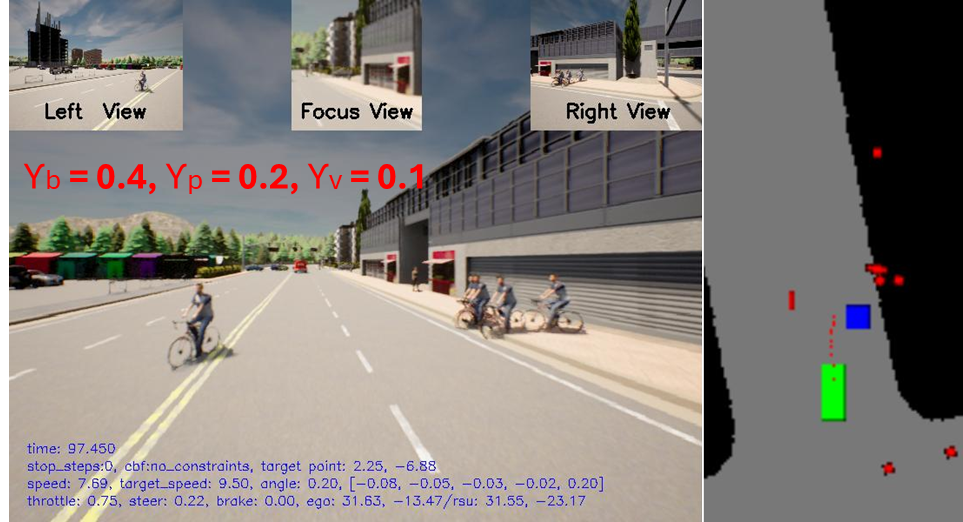
\includegraphics[width=0.23\textwidth]{figures/gamma0_4.png}
}
%\vspace{2mm}
\subfloat[]{
\label{fig:gamma08}
  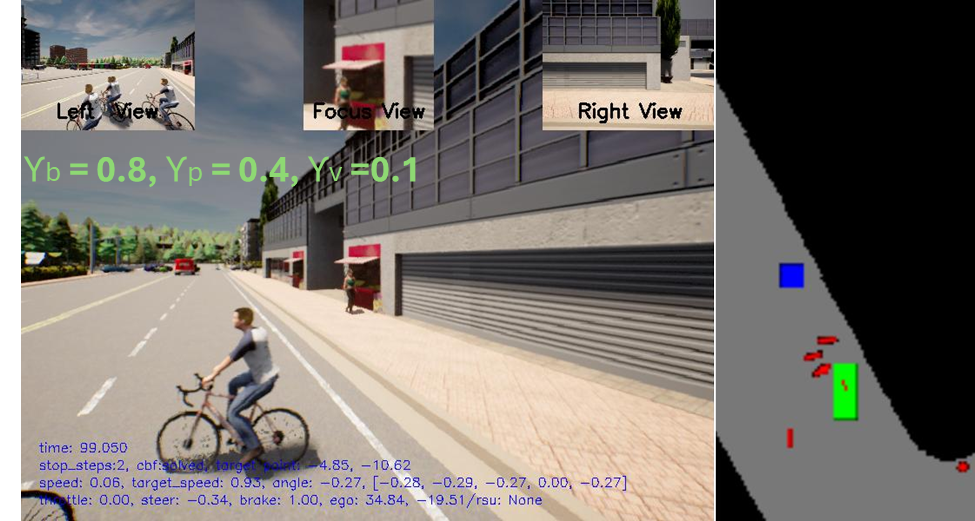
\includegraphics[width=0.23\textwidth]{figures/gamma0_8.png}
}
\caption{Adaptive barrier gains during a cyclist encounter. (a) Bicycles detected ahead, speed 7.69 m/s. (b) Cyclist in the path, so the vehicle stopped.}
\label{fig:gamma-example}
\end{figure}


%------------------------------------------------------------------
\subsection{CBF Filter Parameters}
%------------------------------------------------------------------

Table~\ref{tab:cbf-params} lists the CBF filter parameters. Path-aware gating discards actors behind the rear threshold or outside the lateral corridor, unless their estimated crossing TTC is below the threshold. The speed-dependent corridor term prevents false braking for adjacent-lane traffic.

\begin{table}[!htbp]
\centering
\caption{CBF filter hyperparameters.}
\label{tab:cbf-params}
{\scriptsize
\setlength{\tabcolsep}{5.5pt}
\begin{tabular}{lll}
\toprule
\textbf{Parameter} & \textbf{Symbol} & \textbf{Value} \\
\midrule
Max actor range            & $d_{\max}$        & 30.0\,m \\
Safety margin              & $m$               & 2.5\,m \\
Braking deceleration       & $a_{\text{brake}}$& 6.0\,m/s\textsuperscript{2} \\
Min / max acceleration     & $a_{\min},a_{\max}$ & $-8.0$\,/\,4.0\,m/s\textsuperscript{2} \\
Slack penalty              & $w_s$             & 1000 \\
Control interval           & $\Delta t$        & 0.2\,s \\
Alignment floor            & $\eta_{\text{floor}}$ & 0.15 \\
Max actor accel.\ bound    & $a_i^{\max}$      & 3.0\,m/s\textsuperscript{2} \\
\midrule
\multicolumn{3}{l}{\textit{Path-aware actor gating}} \\
\midrule
Rear ignore distance       &                   & 2.0\,m \\
Lateral corridor half width&                   & 2.5\,m + 0.04\,$v_{\text{ego}}$ \\
Crossing TTC threshold     &                   & 3.2\,s \\
\bottomrule
\end{tabular} }
\end{table}

%------------------------------------------------------------------
\subsection{RL Training Configuration}
%------------------------------------------------------------------

The adaptive gamma policy is trained with constrained PPO (Section~\ref{methods}). Training is on-policy: each iteration collects 2000 decision steps, then performs 10 epochs of minibatch PPO updates with PID-based Lagrangian adjustment. A small entropy bonus ($\alpha_H{=}0.005$) aids early exploration. The actor-critic has $\sim$10k parameters; a full training run of 800k--1M environment steps takes 3--5 days on a single NVIDIA RTX 6000 Ada GPU. Table~\ref{tab:rl-params} lists all hyperparameters.

\begin{table}[!htbp]
\centering
\caption{RL training hyperparameters.}
\label{tab:rl-params}
{\scriptsize
\setlength{\tabcolsep}{5.5pt}
\begin{tabular}{ll}
\toprule
\textbf{Parameter} & \textbf{Value} \\
\midrule
Obs / action dim              & 11 / 3 (one $\gamma$ per class) \\
Hidden layers                 & 2 $\times$ 64, Tanh \\
Learning rate                 & $3 \times 10^{-4}$ \\
$\gamma_{\text{RL}}$\,/\,GAE $\lambda$ & 0.99 / 0.95 \\
PPO clip $\epsilon$           & 0.2 \\
Epochs / minibatches          & 10 / 8 \\
Rollout size                  & 2000 steps \\
$\alpha_H$\,/\,$\alpha_V$\,/\,grad clip & 0.005 / 0.5 / 0.5 \\
\midrule
\multicolumn{2}{l}{\textit{Constrained optimization}} \\
\midrule
Cost limit $c_{\text{limit}}$   & 0.1 \\
PID $(k_p, k_i, k_d)$\,/\,EMA $\alpha$ & (1.0, 0.1, 0.1)\,/\,0.9 \\
$\lambda_{\max}$              & 100.0 \\
$c_{\text{col}}$ (terminal)   & 3.0 \\
$[\gamma_{\min},\,\gamma_{\max}]$ all classes & [0.05, 0.8] \\
\bottomrule
\end{tabular} }
\end{table}

%------------------------------------------------------------------
\subsection{Baselines}
%------------------------------------------------------------------

We compare three longitudinal control configurations that share frozen perception, planning, and lateral control:

%\begin{enumerate}
    %\item 
\textbf{No CBF}: Raw planner output passes to the unfiltered actuator (unmodified V2Xverse stack).
    %\item 

\textbf{Fixed CBF}: CBF-QP with constant $\gamma_v{=}\gamma_p{=}\gamma_b{=}0.5$, selected based on preliminary experiments that indicated that this value balanced safety and route completion.
    %\item 
    
\textbf{Adaptive CBF}: CBF-QP with class-specific $\gamma$ values in $[0.05,0.8]$ selected per step by the trained RL policy.
%\end{enumerate}

\subsubsection{Checkpoint Selection}
\label{sec:checkpoint-selection}
The checkpoint underlying the results reported in Section~\ref{results} was selected using the evaluator's original best-checkpoint logic, which scored candidate checkpoints against cumulative statistics computed over the same route pool used for final reporting, rather than a disjoint held-out set. We have since corrected this: candidate checkpoints are now scored only against a designated validation subset of routes, held out from both the training rollout stream and the final test set, before a checkpoint is selected for reporting. This validation-gating fix is implemented and verified on synthetic checkpoint records, but regenerating the headline checkpoint under the corrected procedure requires a full retraining run, which was not completed in time for this submission. We report this directly rather than leave it unstated, and treat producing a validation-selected checkpoint as the top priority for the next iteration of this work.

%------------------------------------------------------------------
\subsection{Evaluation Protocol and Metrics}
%------------------------------------------------------------------

All methods are evaluated in deterministic mode (mean policy action) on the same Town05 routes with fixed random seeds. Multiple passes per method account for the residual nondeterminism of CARLA. We report the standard CARLA leaderboard driving score,
\begin{equation}
\text{score} = \text{score}_{\text{route}} \times \text{score}_{\text{penalty}},
\end{equation}
where $\text{score}_{\text{route}}$ is the percentage of the route completed and $\text{score}_{\text{penalty}}$ starts at 1.0 and is multiplied by a fixed weight for every infraction incurred: $\times0.50$ for a pedestrian collision, $\times0.60$ for a vehicle collision, $\times0.65$ for a static-object collision, $\times0.70$ for running a red light, $\times0.80$ for a stop-sign violation, and a factor scaled by the percentage of the route driven outside the lane for off-route driving. We additionally report the route score, the route completion rate (fraction of trials where the full route was finished), collisions per route and per kilometer (split by actor class: vehicle, bicycle, pedestrian, static), and the collision-free route fraction. A method is considered an improvement if it reduces collision rates without a proportional loss in route completion.

%------------------------------------------------------------------
\subsection{Additional Ablations and Robustness Probes}
\label{sec:additional-ablations}
%------------------------------------------------------------------

Beyond the three-way baseline comparison above, we conduct the following additional experiments, with results reported in Section~\ref{results}.

\textbf{Fixed-gain sensitivity sweep.} We evaluate the fixed-CBF baseline at eight values, $\gamma \in \{0.1, 0.2, \dots, 0.8\}$, each over the full 105-route Town05 set, to test whether the adaptive policy's advantage depends on an unfavorable choice of static gain.

\textbf{Cross-map generalization.} The trained adaptive policy is evaluated zero-shot, with no retraining, on two towns never seen during training or the main evaluation: Town07 (42 trials) and Town10 (27 trials).

\textbf{Collaboration ablation.} We re-evaluate the identical trained safety layer wrapped around V2Xverse's single-agent (\texttt{no\_collaboration}) perception-planning checkpoint in place of the collaborative \texttt{codriving} checkpoint, holding the safety layer fixed, over the full 105-route set. The CBF filter and RL policy observation are built from ground-truth CARLA actor state rather than either perception model's own detections, so this isolates the upstream planner's use of collaboration rather than the safety layer's own dependence on it.

\textbf{Rule-based scheduler baseline.} We compare against a hand-designed, non-learned $\gamma$ scheduler that ramps linearly with time-to-collision per actor class, requiring no training or checkpoint, over the full 105-route set.

\textbf{Class-specific vs.\ shared gain.} A full ablation would retrain a policy constrained to a single shared $\gamma$ across all actor classes. As a lower-cost, training-free proxy, we instead log the trained class-specific policy's three per-class gains over a 20-route subset and measure how much they diverge from one another in deployment, which is suggestive of reliance on class-specific information but does not establish that a shared-gain policy would perform worse if trained under that constraint.

\textbf{Observation-space sensitivity.} As a similarly training-free proxy for an observation-space ablation, we mask the heading-alignment features from the trained policy's input at inference time (on the same 20-route subset) and measure the resulting change in driving performance. As with the class-specific-gain proxy, this measures the deployed policy's sensitivity to losing an input it was trained to expect, which is not equivalent to training a policy that never had access to that feature.

\textbf{Traffic density and V2X robustness.} On a 20-route subset, we evaluate the adaptive policy under $1.5\times$ denser background traffic, under injected V2X communication latency (400\,ms), and under injected collaborative-perception pose noise ($\sigma_{\text{pos}}=\sigma_{\text{rot}}=0.2$), each individually, to probe sensitivity to conditions beyond the default evaluation setting. These are single-condition probes at one severity level rather than full sweeps.
\section{Results}
\label{results}

All three methods are evaluated over 315 route trials on Town05. Table~\ref{tab:main-results} summarizes the aggregate metrics, while Figs.~\ref{fig:collision-breakdown}--\ref{fig:infraction-breakdown} visualize the score distributions and per-class collision breakdown.

\begin{table*}[!htbp]
\centering
\caption{Aggregate evaluation results on Town05 (315 trials each; driving score shown with 95\% CI). Collision columns are split by actor class: vehicles, bicycles, and pedestrians.}
\label{tab:main-results}
{\scriptsize
\setlength{\tabcolsep}{5.5pt}
\begin{tabular}{lcccccccccc}
\toprule
\textbf{Method}
  & \makecell{\textbf{Driving}\\\textbf{Score\,$\uparrow$}}
  & \makecell{\textbf{Route}\\\textbf{Score\,$\uparrow$}}
  & \makecell{\textbf{Route}\\\textbf{Compl.\,$\uparrow$}}
  & \makecell{\textbf{Coll.}\\\textbf{/Route\,$\downarrow$}}
  & \makecell{\textbf{Coll.}\\\textbf{/km\,$\downarrow$}}
  & \makecell{\textbf{Coll.}\\\textbf{Free\,$\uparrow$}}
  & \makecell{\textbf{Veh.}\\\textbf{/Rt\,$\downarrow$}}
  & \makecell{\textbf{Bike}\\\textbf{/Rt\,$\downarrow$}}
  & \makecell{\textbf{Ped.}\\\textbf{/Rt\,$\downarrow$}}
  & \makecell{\textbf{Static}\\\textbf{/Rt\,$\downarrow$}} \\
\midrule
PID-only
  & 45.47\,($\pm$4.41)
  & 96.91
  & 90.2\%
  & 2.952
  & 35.58
  & 31.7\%
  & 0.968
  & 1.527
  & 0.390
  & 0.067 \\
Fixed CBF
  & 67.39\,($\pm$3.58)
  & 95.36
  & 88.3\%
  & 0.784
  & 9.56
  & 48.6\%
  & 0.168
  & 0.286
  & 0.302
  & 0.029 \\
\textbf{Adaptive CBF}
  & \textbf{75.81}\,($\pm$3.35)
  & 96.71
  & \textbf{90.8\%}
  & \textbf{0.581}
  & \textbf{6.75}
  & \textbf{59.7\%}
  & 0.187
  & \textbf{0.187}
  & \textbf{0.178}
  & 0.029 \\
\bottomrule
\end{tabular} }
\end{table*}

%------------------------------------------------------------------
\subsection{Safety Analysis}
%------------------------------------------------------------------

As shown in Table~\ref{tab:main-results}, the adaptive CBF policy scores 75.81\,($\pm$\,3.35) on the driving metric and produces the fewest collisions across bicycles and pedestrians. Relative to PID-only, total collisions per route drop by 80.3\% (2.952 to 0.581), and collisions per kilometer by 81.0\% (35.58 to 6.75), with bicycles seeing the steepest reduction at 87.7\% (1.527 to 0.187). Vehicle and pedestrian collisions fall by 80.7\% (0.968 to 0.187) and 54.5\% (0.390 to 0.178), respectively.


The adaptive policy further improves on the fixed CBF baseline, cutting collisions per route by 25.9\% (0.784 to 0.581) and collisions per kilometer by 29.3\% (9.56 to 6.75). Most of this improvement comes from pedestrians (41.1\% lower) and bicycles (34.4\% lower), which aligns with the design intent: the RL policy raises $\gamma_p$ and $\gamma_b$ when vulnerable road users approach the ego trajectory, braking more aggressively only when it matters. The collision-free route rate rises from 48.6\% under fixed CBF to 59.7\% under the adaptive CBF. Fig.~\ref{fig:collision-breakdown} shows the per-class breakdown. PID-only's total is dominated by bicycle collisions, which account for over half of its bar. Both CBF methods reduce bicycle and vehicle collisions substantially, bringing those categories to comparable levels. The adaptive policy then separates itself from the fixed variant primarily through lower pedestrian collisions, consistent with its ability to tighten $\gamma$ when vulnerable road users are nearby.


%------------------------------------------------------------------
\subsection{Efficiency Analysis}
%------------------------------------------------------------------

Despite being more conservative on safety, the adaptive policy does not sacrifice route progress. It slightly edges out PID-only route completion (90.8\% vs.\ 90.2\%), while fixed CBF completes only 88.3\%. The fixed gain tends to over-brake in tight gaps, stalling the vehicle; the adaptive policy avoids this by relaxing $\gamma$ when no hazard is nearby, so it records only 24 blocked-agent failures versus 35 for fixed CBF and 31 for PID-only. The penalty factor (driving score divided by route score) captures how cleanly routes are completed: 0.784 for adaptive policy, 0.707 for fixed CBF, and 0.469 for PID-only. In other words, PID-only loses more than half its route score to infraction penalties on an average run.


%------------------------------------------------------------------
\subsection{Score Distribution}

%------------------------------------------------------------------

The violin plots in Fig.~\ref{fig:overall-scores} give a fuller picture than the averages alone. The black line represents the mean, and the red line represents the median. More than half of the adaptive CBF routes (56.2\%) score a perfect 100, pulling the median to 100.0. Fixed CBF sits at a median of 60.0 and PID-only at 30.0; the latter shows a heavy lower tail with 85 routes below a score of 10, each flagging an early collision that dominates the final penalty. The tighter interquartile range for adaptive policy ($[50, 100]$ versus $[8, 100]$ for PID-only) suggests that improvement holds in a wide variety of route layouts rather than being concentrated on a few easy ones. Route-level paired comparisons support this: the adaptive policy outscores PID-only on 64.4\% of routes (worse on only 7.9\%) and beats fixed CBF on 36.2\% (worse on 18.7\%).

%------------------------------------------------------------------
\subsection{Infraction Breakdown}
%------------------------------------------------------------------

Fig.~\ref{fig:infraction-breakdown} breaks down the mean infractions per route in the five categories shown. Bicycle infractions are the largest for PID-only at 1.527 per route; fixed CBF reduces this to 0.286, and the adaptive policy to 0.187. Vehicle infractions follow a similar trend: 0.968 for PID-only, 0.168 for fixed CBF, and 0.187 for adaptive. Pedestrian infractions drop from 0.390 (PID-only) to 0.302 (fixed CBF) and 0.178 (adaptive). Static object infractions are low across the board -- 0.067, 0.029, and 0.029 for PID-only, fixed CBF, and adaptive, respectively. Stop-sign infractions round out the picture at 0.248 for PID-only, 0.235 for fixed CBF, and 0.168 for the adaptive policy.


\begin{figure}[!htbp]
  \centering
  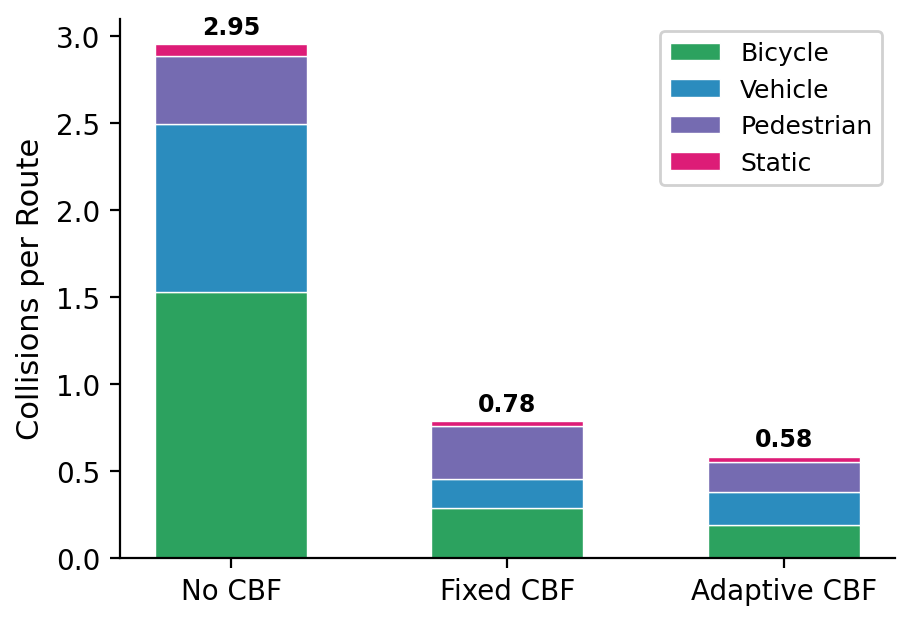
\includegraphics[width=0.5\columnwidth]{figures/collision_breakdown.png}
  \caption{Mean collisions per route, stacked by actor class.}
  \label{fig:collision-breakdown}
\end{figure}

\begin{figure}[!htbp]
  \centering
  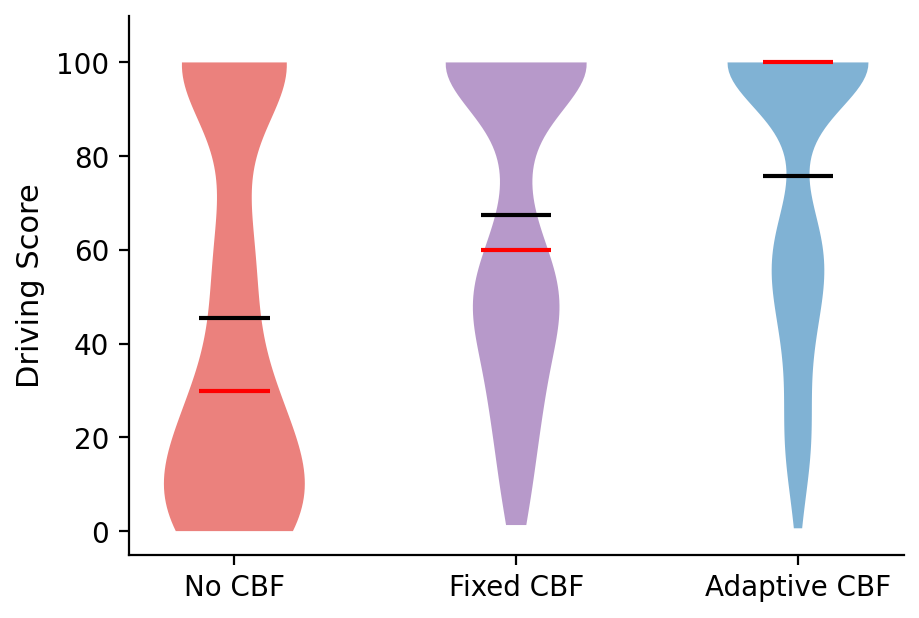
\includegraphics[width=0.5\columnwidth]{figures/score_distribution.png}
  \caption{Per-route driving score distributions.}
  \label{fig:overall-scores}
\end{figure}



\begin{figure}[!htbp]
  \centering
  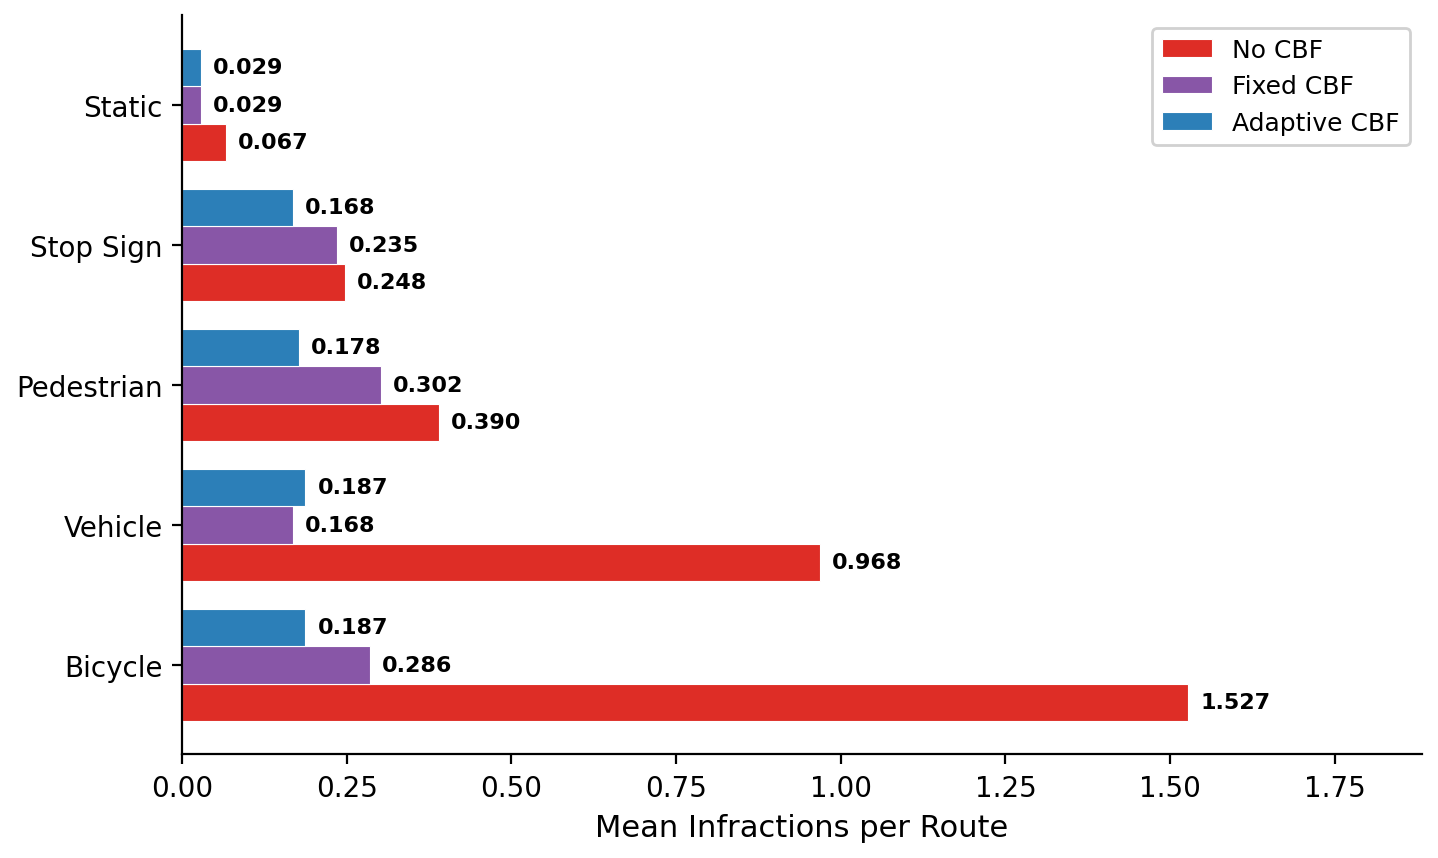
\includegraphics[width=0.9\columnwidth]{figures/all_infractions_per_route.png}
  \caption{Mean infractions per route by category.}
  \label{fig:infraction-breakdown}
\end{figure}

%------------------------------------------------------------------
\subsection{Execution Time and Constraint Activation}
\label{sec:solve-time}
%------------------------------------------------------------------

Across the full evaluation matrix ($\sim$42k decision steps per method), the OSQP solve for a single decision step averages $0.017$\,ms (95th percentile $0.041$\,ms, maximum $<\!1.1$\,ms), against the $200$\,ms budget imposed by the $5$\,Hz decision rate -- solve time consumes under $0.02\%$ of the available budget on average, well within real-time requirements even in dense traffic. The QP's slack variable is active on $30.4\%$ of decision steps for the fixed-gain baseline and $35.2\%$ for the adaptive policy, indicating the soft constraint is exercised regularly rather than only in rare edge cases; the solver never fell back to the nominal (unfiltered) command in either case ($0.0\%$ fallback rate across both methods), so feasibility was never lost even under the one-step linearization discussed in Section~\ref{methods}.

%------------------------------------------------------------------
\subsection{Fixed-Gain Sensitivity Sweep}
\label{sec:gamma-sweep}
%------------------------------------------------------------------

Table~\ref{tab:gamma-sweep} sweeps the fixed-CBF gain across its full configured range. The eight fixed-gain points span only $66.55$--$71.75$, a band narrower than any individual point's own 95\% CI ($\pm6.2$--$6.6$) -- no fixed gain is statistically distinguishable from any other, indicating the fixed-CBF baseline was not tuned to an unfavorable operating point. At matched sample size ($\gamma{=}0.5$ vs.\ adaptive, both $n{=}315$), the adaptive policy's advantage is real but modest: $75.81\pm3.35$ vs.\ $67.39\pm3.58$, confidence intervals barely non-overlapping. Fig.~\ref{fig:gamma-pareto} plots this as a Pareto frontier.

\begin{table}[!htbp]
\centering
\caption{Fixed-CBF gamma sensitivity sweep, Town05 ($n{=}105$ per point except $\gamma{=}0.5$, $n{=}315$).}
\label{tab:gamma-sweep}
{\scriptsize
\setlength{\tabcolsep}{4pt}
\begin{tabular}{lcccc}
\toprule
$\gamma$ & Score & 95\% CI & Compl. & Coll./km \\
\midrule
0.1 & 67.76 & 6.51 & 90.5\% & 10.76 \\
0.2 & 69.64 & 6.23 & 88.6\% & 8.98 \\
0.3 & 67.55 & 6.22 & 88.6\% & 8.95 \\
0.4 & 71.75 & 6.31 & 86.7\% & 8.49 \\
0.5 & 67.39 & 3.58 & 88.3\% & 9.56 \\
0.6 & 66.57 & 6.65 & 86.7\% & 11.46 \\
0.7 & 70.54 & 6.42 & 89.5\% & 9.42 \\
0.8 & 66.55 & 6.62 & 89.5\% & 10.43 \\
\textbf{Adaptive} & \textbf{75.81} & 3.35 & 90.8\% & 6.75 \\
\bottomrule
\end{tabular} }
\end{table}

\begin{figure}[!htbp]
  \centering
  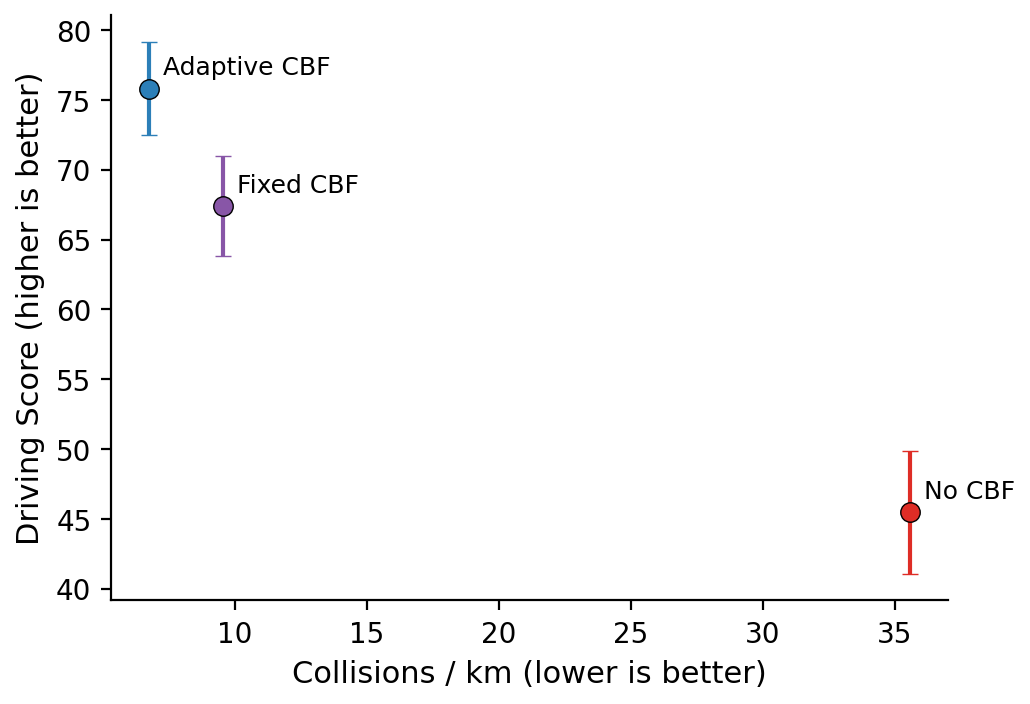
\includegraphics[width=0.9\columnwidth]{figures/pareto_score_vs_collisions.png}
  \caption{Fixed-CBF gamma sweep: score vs.\ collision rate, adaptive CBF shown as reference.}
  \label{fig:gamma-pareto}
\end{figure}

%------------------------------------------------------------------
\subsection{Cross-Map Generalization}
\label{sec:generalization}
%------------------------------------------------------------------

Table~\ref{tab:generalization} evaluates the frozen trained policy zero-shot on two held-out towns. The CBF-vs-no-CBF safety benefit holds cleanly across all three towns: PID-only's collision rate rises sharply out of distribution ($35.58\rightarrow99.57\rightarrow66.13$ per km) while both CBF variants remain in a comparatively narrow band. The adaptive-over-fixed advantage observed on Town05, however, does not generalize: the two are statistically indistinguishable on Town07, and fixed CBF outperforms the adaptive policy on Town10 on both score and collision rate. We report this directly: the safety-layer concept generalizes, but the specific claim that adaptive scheduling outperforms a well-tuned fixed gain is currently supported only in-distribution.

\begin{table}[!htbp]
\centering
\caption{Cross-map generalization, zero-shot (no retraining).}
\label{tab:generalization}
{\scriptsize
\setlength{\tabcolsep}{4pt}
\begin{tabular}{lccc}
\toprule
Method & Town05 ($n{=}315$) & Town07 ($n{=}42$) & Town10 ($n{=}27$) \\
\midrule
PID-only score      & 45.47$\pm$4.4  & 23.46$\pm$9.8 & 17.33$\pm$11.4 \\
Fixed CBF score      & 67.39$\pm$3.6  & 71.50$\pm$8.2 & 43.27$\pm$12.6 \\
Adaptive CBF score   & 75.81$\pm$3.4  & 72.86$\pm$8.9 & 38.41$\pm$12.6 \\
\midrule
PID-only coll./km    & 35.58 & 99.57 & 66.13 \\
Fixed CBF coll./km   & 9.56  & 9.50  & 14.37 \\
Adaptive CBF coll./km& 6.75  & 9.26  & 20.97 \\
\bottomrule
\end{tabular} }
\end{table}

%------------------------------------------------------------------
\subsection{Ablation Studies}
\label{sec:ablations}
%------------------------------------------------------------------

\textbf{Collaboration ablation.} Wrapping the identical safety layer around the single-agent (\texttt{no\_collaboration}) perception-planning checkpoint scores $67.57\pm6.52$, $89.5\%$ completion, $10.91$ collisions/km ($n{=}105$), versus $75.81\pm3.35$, $90.8\%$, $6.75$ with collaborative perception. The safety layer still delivers a large improvement over the unfiltered baseline without collaboration, but collaborative perception provides a further, meaningful benefit on top of it -- the reported gains are not solely an artifact of collaboration.

\textbf{Rule-based scheduler baseline.} Table~\ref{tab:rule-based} compares the hand-designed TTC-ramp scheduler against the other three methods. The ordering is monotonic on both score and collision rate: rule-based clearly beats no safety layer, but underperforms even the simplest fixed-gain CBF, and more so the learned adaptive policy -- the learned policy earns its added complexity over a simple hand-tuned rule.

\begin{table}[!htbp]
\centering
\caption{Rule-based (non-learned) gamma-scheduler baseline, Town05.}
\label{tab:rule-based}
{\scriptsize
\setlength{\tabcolsep}{4pt}
\begin{tabular}{lcccc}
\toprule
Method & $n$ & Score & Compl. & Coll./km \\
\midrule
PID-only        & 315 & 45.47$\pm$4.41 & 90.2\% & 35.58 \\
Rule-based CBF  & 105 & 64.46$\pm$6.76 & 89.5\% & 12.80 \\
Fixed CBF       & 315 & 67.39$\pm$3.58 & 88.3\% & 9.56 \\
Adaptive CBF    & 315 & 75.81$\pm$3.35 & 90.8\% & 6.75 \\
\bottomrule
\end{tabular} }
\end{table}

\textbf{Class-specific gain and observation-space proxies.} These are training-free proxies, not controlled ablations (Section~\ref{sec:additional-ablations}); we report them as such. Logging the trained policy's three gains over 6{,}485 decision steps shows they do not converge to a shared value: mean pairwise gaps of $0.60$--$0.63$ between the pedestrian gain and the other two classes, with $0\%$ of steps landing all three gains within even $0.10$ of each other -- the deployed policy clearly exploits class-specific freedom, particularly for pedestrians, though this does not establish that a policy trained under a shared-gain constraint could not perform comparably. One class's mean gain ($\gamma_v{=}0.800$, the top of the configured range) has exactly zero measured variance across all logged steps, which we note as a possible sign that this action dimension saturated during training rather than learning to differentiate, and flag as worth further investigation rather than presenting as a clean result. Separately, masking the heading-alignment features at inference dropped mean score from $67.73$ to $63.10$ and raised collisions from 14 to 18 over the same 20 routes, a real but noisy effect (6 routes worse, 4 better, 10 unchanged) consistent with the policy relying on this feature to some degree, though it cannot separate that from sensitivity to an out-of-distribution input.

%------------------------------------------------------------------
\subsection{Traffic Density and V2X Robustness}
\label{sec:robustness}
%------------------------------------------------------------------

On a 20-route subset (baseline: score $67.73$, $95\%$ completion, 14 collisions), $1.5\times$ denser traffic reduces the adaptive policy to score $61.09$, $70\%$ completion, 18 collisions -- a real degradation under harder conditions, as expected. Injected V2X communication latency ($400$\,ms) and collaborative-perception pose noise ($\sigma_{\text{pos}}{=}\sigma_{\text{rot}}{=}0.2$), tested individually, did not degrade score relative to baseline ($69.23$ and $73.42$ respectively). We report this as a single data point per condition rather than a sweep to a breaking point, and do not claim broad robustness from it alone.

\FloatBarrier
\section{Conclusion}
\label{Conclusion}

This paper introduces an adaptive CBF safety layer for collaborative autonomous driving that works with the V2Xverse CoDriving stack without retraining perception or planning. By adapting only the safety enforcement while keeping upstream modules fixed, our approach ensures that observed improvements are attributable to the safety layer, suggesting its portability and ease of integration into other collaborative driving platforms.

The approach combines a modular CBF-QP safety filter with a class-aware adaptive $\gamma$ policy trained using constrained PPO and a PID-based Lagrangian. A compact network outputs gains per-step for vehicles, pedestrians, and bicycles from traffic-risk features, while the CBF remains the final mechanism that enforces bounded longitudinal actions. This keeps the safety layer interpretable, lightweight, and directly compatible with an existing collaborative autonomy stack.

When evaluated in Town05 against PID-only and fixed CBF under the same perception, planning, and steering setup, the adaptive method delivered the strongest overall performance: driving score $75.81 \pm 3.35$, collisions per route 0.581, and collisions per kilometer 6.75. Relative to PID-only, collisions per route dropped by 80.3\%, and relative to fixed CBF, they dropped by 25.9\%. The completion of the route remained high at 90.8\%, while the collision-free route rate increased to 59.7\%. The greatest gains on bicycles and pedestrians show that adaptive gain scheduling is especially useful for vulnerable road users in heterogeneous traffic.

Overall, these results support the central claim of the paper: learning to schedule barrier gains online can improve safety without sacrificing route progress. More broadly, they show that meaningful safety improvements can come from a targeted control-layer intervention rather than a full redesign of the autonomy stack.

\textbf{Limitations.} Our formulation does not provide a formal forward-invariance guarantee. The slack variable in the QP admits soft constraint violation when the problem would otherwise be infeasible, and we measure it as active on $30$--$35\%$ of decision steps (Section~\ref{sec:solve-time}); the solver never fell back to the nominal command, but this means the safety property is empirical rather than certified. We bound, rather than eliminate, the risk from the constant-velocity actor assumption via a worst-case acceleration margin (Section~\ref{methods}), and our barrier formulation acts on longitudinal motion only: extending the framework to jointly regulate longitudinal and lateral actions is a natural next step, requiring a coupled vehicle model and richer barrier construction. The checkpoint underlying our headline result predates the checkpoint-selection methodology fix described in Section~\ref{sec:checkpoint-selection}; producing a validation-selected headline result is the top priority for future work. Finally, three additional ablations explicitly called for could not be completed with a trained policy in this revision cycle and remain future work: class-specific-vs-shared-gain and cost-function-weighting variants, and a PID-Lagrangian-vs-plain-Lagrangian comparison -- each requires training a separate policy under the corresponding constraint, which we substituted where possible with training-free proxies on the existing policy (Section~\ref{sec:ablations}) rather than presenting as equivalent evidence. Even with these limitations, the approach is practical as a drop-in safety adapter for existing autonomy stacks and complements continued advances in collaborative perception and planning.


                                  % sure that you do not shorten the textheight too much.

%%%%%%%%%%%%%%%%%%%%%%%%%%%%%%%%%%%%%%%%%%%%%%%%%%%%%%%%%%%%%%%%%%%%%%%%%%%%%%%%



%%%%%%%%%%%%%%%%%%%%%%%%%%%%%%%%%%%%%%%%%%%%%%%%%%%%%%%%%%%%%%%%%%%%%%%%%%%%%%%%



%%%%%%%%%%%%%%%%%%%%%%%%%%%%%%%%%%%%%%%%%%%%%%%%%%%%%%%%%%%%%%%%%%%%%%%%%%%%%%%%
%\section*{APPENDIX}

%Appendixes should appear before the acknowledgment.

\section*{ACKNOWLEDGMENT}
%The authors acknowledge funding from NSF CREST Center for Multidisciplinary Research Excellence in Cyber-Physical Infrastructure Systems (No. 2112650). NSF CISE MSI programs (No. 2318682 $\&$ 2431569) and NSF CISE Expand AI Program (No. 2434916).


%%%%%%%%%%%%%%%%%%%%%%%%%%%%%%%%%%%%%%%%%%%%%%%%%%%%%%%%%%%%%%%%%%%%%%%%%%%%%%%%

%References are important to the reader; therefore, each citation must be complete and correct. If at all possible, references should be commonly available publications.

\bibliographystyle{IEEEtran}
\bibliography{BibFiles/IEEEabrv, BibFiles/main_ref}

\end{document}
